\subsubsection{Catalog Page Specifications}
The catalog page is where the user can view their already processed data stored in the backend. If this user is using a shared server, this can potentially also show processed data from \textit{other} users in their group, should those permissions be allowed.\par
The catalog page will be depicted in two separate views, the first involving searching, filtering and selecting jobs and the second, viewing visualizations for the results of the selected jobs. It will usually be the case that users will create a large amount of jobs, corresponding to sets of sound files captured at various locations. Therefore, filtering jobs will be a necessary feature when selecting job results to analyze. The core functionality of the first view is as follows:\\
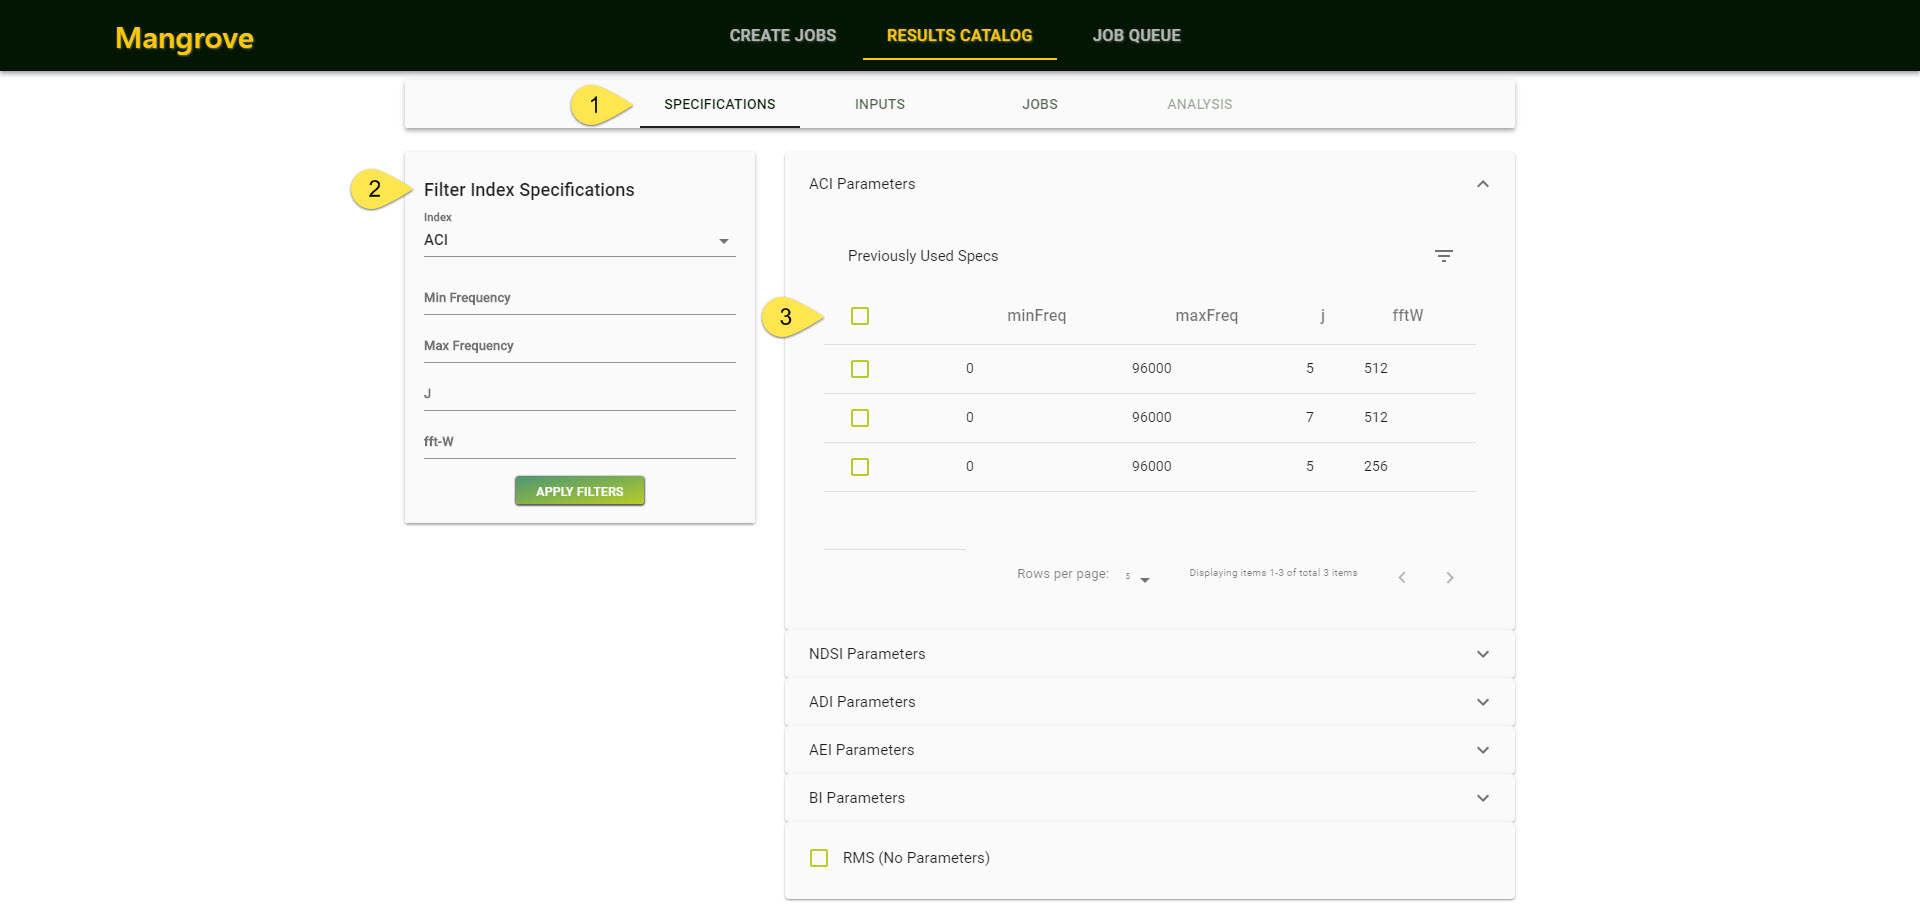
\includegraphics[width=\textwidth]{catalog-1}
\begin{enumerate}
    \item \textbf{Job Searching}\\ The user can search for jobs by site name or tags, which the user can apply to one or many jobs. This feature is helpful if the user wishes to compare results of sound files taken in the same location. An example of searching by a site name, such as \textquotesingle UCF Arboretum\textquotesingle , would show all files captured at that location, provided the user has given the site name as input. Tags will be used to group files in any way that will be relevant to the researcher.
    \item \textbf{Filter By Index}\\ This section consists of a set of checkboxes for each index. They will all be selected when this page is loaded, so that all jobs will be shown to the user at first. Users can uncheck indices as they wish, so that only jobs which were run with checked indices will be listed. Combined with job searching, a user could view results of jobs on files taken in the same location, but analyzed with different indices.
    \item \textbf{Filter By Parameters}\\ This is where a user can specify the parameters used for the jobs which they would like to view analysis. Only parameters for checked indices will be displayed. An example of the usefulness of this feature is when a researcher would like to compare results analyzed within certain frequency ranges.
    \item \textbf{Sorting By Date}\\ Jobs matching the criteria set by the user in the previous sections will be listed with the most recently analyzed jobs shown first. However, the user will be able to show the oldest jobs first or input a specific date range.
    \item \textbf{Filtered Jobs}\\ This is where all jobs matching the filtering and searching done by the user will be listed.
    \item \textbf{View Results}\\ When the user finds the job they would like to visualize, they will click the 'view results' button next to that job. This will open the analysis view of the catalog page and the searching and filtering section will be hidden to allow more room for visualizations.
\end{enumerate}
Some variations to these features will happen if a user belongs to a research group. An option of filtering by jobs that they have created themselves verses themselves and members of their group would be shown. Searching for jobs created by a specific group member would also be permitted in the Job Searching feature.\par
The second view or analysis view of the catalog page focusses on having a clear way for users to view meaningful visualizations of their sound files. The features of the analysis view of the catalog page are outlined below.\par
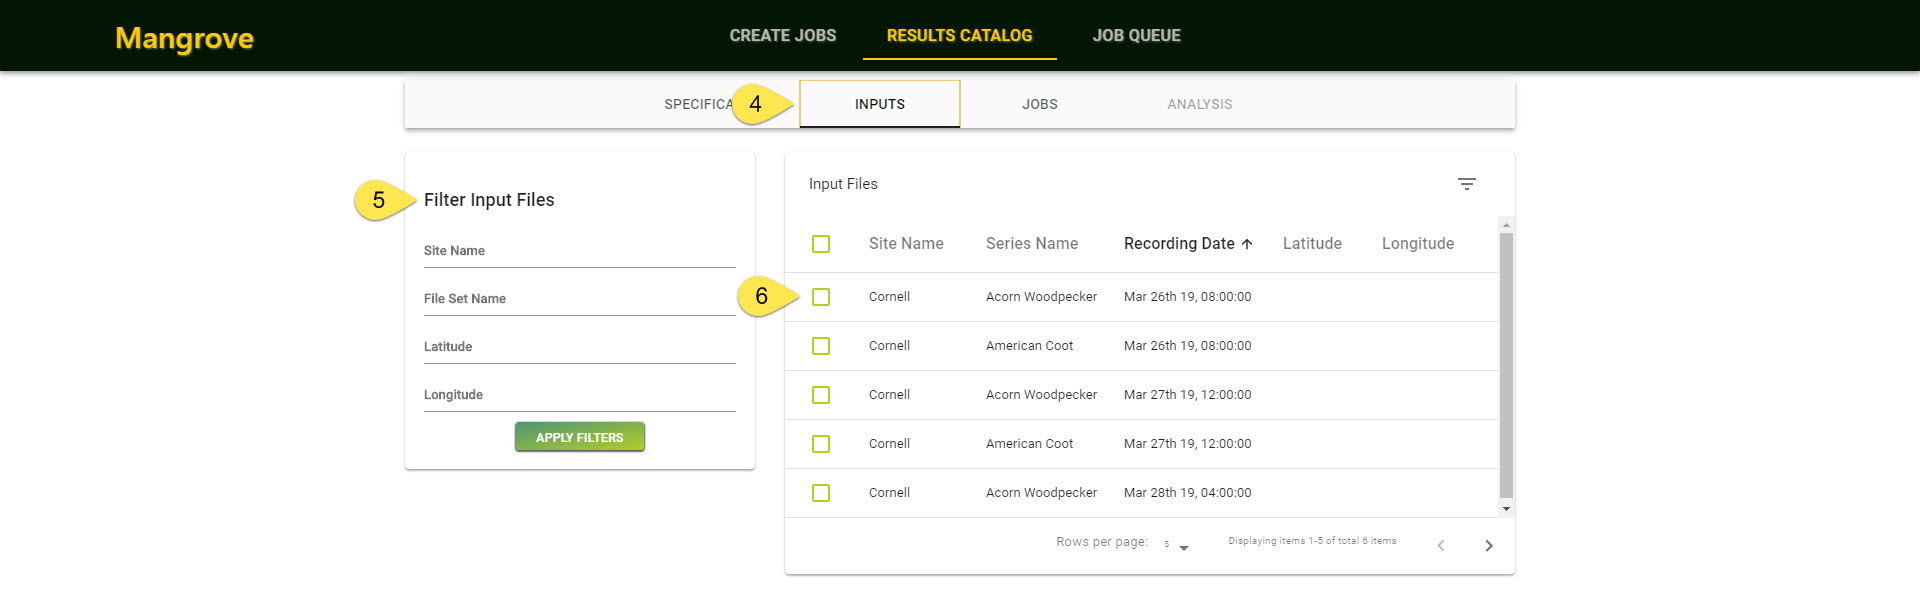
\includegraphics[width=\textwidth]{catalog-2}
\begin{enumerate}
    \item \textbf{Show Filtering Section}\\ If the user wishes to redefine their specifications for the job list, this button can be clicked and will open the previous view.
    \item \textbf{Filtered Jobs}\\ The list of jobs matching the search and filtering specifications set by the user will still be displayed in this view. This section will only take up some of the room on the page and will make the next feature described much easier for users.
    \item \textbf{Compare}\\ If another job of the same index is shown in the filtered job list, the user can click the compare button next to the job. This will overlay both results on the same graph, a feature which will be very useful to researchers.
    \item \textbf{Graph Type Selection}\\ Depending on the parameters and index that was processed, different visualizations will be available. All graphs available for the current index will be listed in this section with radio buttons and the user can select their preferred graph or switch between views.
    \item \textbf{Clear Job}\\ This button can be clicked if the user is finsished viewing the current job\textquotesingle s visualizations. The filtering section will be opened again so a new job can be quickly chosen.
    \item \textbf{View Results}\\ This is where the analysis from the job is shown. Depending on the parameters and index that was processed, different visualizations will be available. If multiple jobs are selected, then a visualization comparing them will be shown.
\end{enumerate}